\documentclass[12pt]{article}

\usepackage[a4paper, margin=1in]{geometry}

\usepackage{listings}
\usepackage{color}
\usepackage{float}
\usepackage{graphicx}
\usepackage{subcaption}

\definecolor{codegreen}{rgb}{0,0.6,0}
\definecolor{codegray}{rgb}{0.5,0.5,0.5}
\definecolor{codepurple}{rgb}{0.58,0,0.82}
\definecolor{backcolour}{rgb}{0.95,0.95,0.92}

\lstdefinestyle{mystyle}{
  backgroundcolor=\color{backcolour},
  commentstyle=\color{codegreen},
  keywordstyle=\color{magenta},
  numberstyle=\tiny\color{codegray},
  stringstyle=\color{codepurple},
  basicstyle=\ttfamily,
  breakatwhitespace=false,
  breaklines=true,
  captionpos=b,
  keepspaces=true,
  numbers=left,
  numbersep=5pt,
  showspaces=false,
  showstringspaces=false,
  showtabs=false,
  tabsize=2
}

\lstset{style=mystyle}

\setlength\parindent{0pt}
\setlength\parskip{1em}

\title{Lab 9 - Gather}
\author{\textsc{Nguyen} Duc Tung}
\date{}

\begin{document}

\maketitle

This lab objective is to do a histogram equalization of greyscale image.
\\\\
I wrote 3 kernels for this task.

\begin{itemize}
  \item First kernel for computing the Histogram of the image
  \item Second kernel for building a map from the range [0, 255] to a new value using the given method. Each thread calculate the new greyscale level of one value in the range [0, 255] (256 threads in total)
  \item Last kernel simply map all pixels to a new value using the map from second kernel
\end{itemize}

Here is the final result, you can clearly see the higher constrast on the sky:

Time elapsed: 25.5 ms

\begin{figure}[H]
  \centering
  \begin{subfigure}{.45\textwidth}
    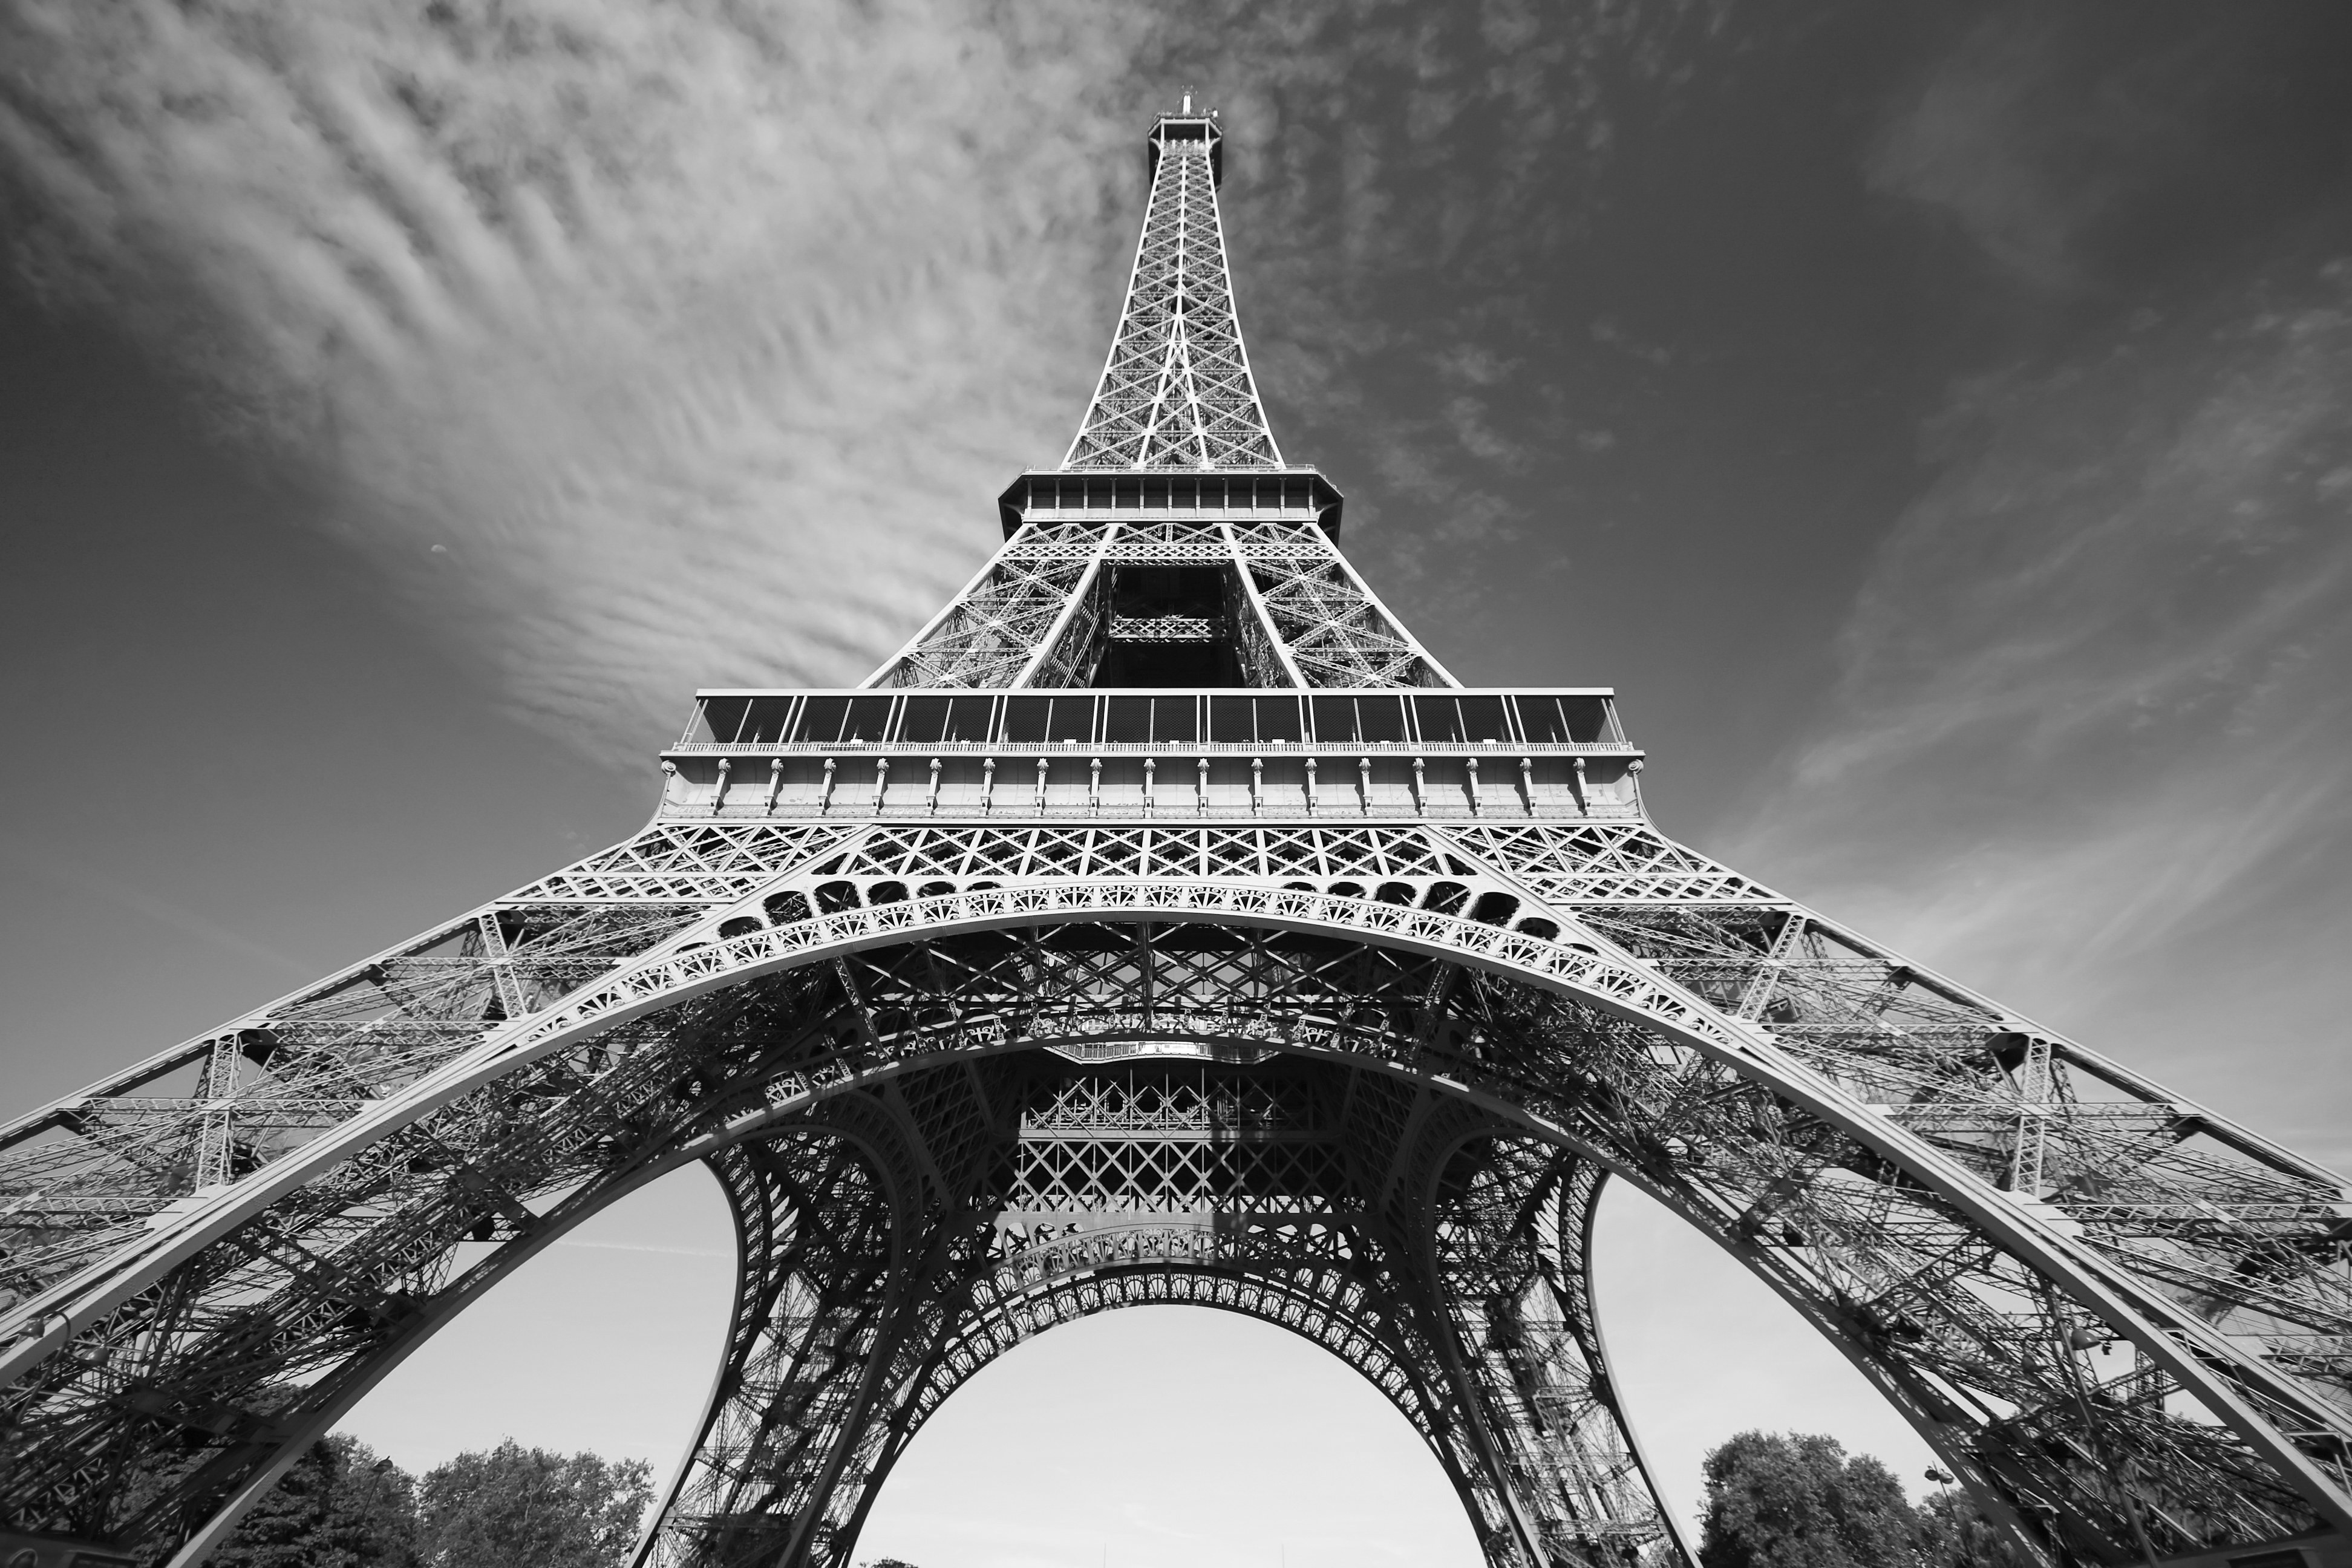
\includegraphics[width=\linewidth]{./img/in.jpg}
    \caption{Original image}
  \end{subfigure}
  \hspace{1cm}
  \begin{subfigure}{.45\textwidth}
    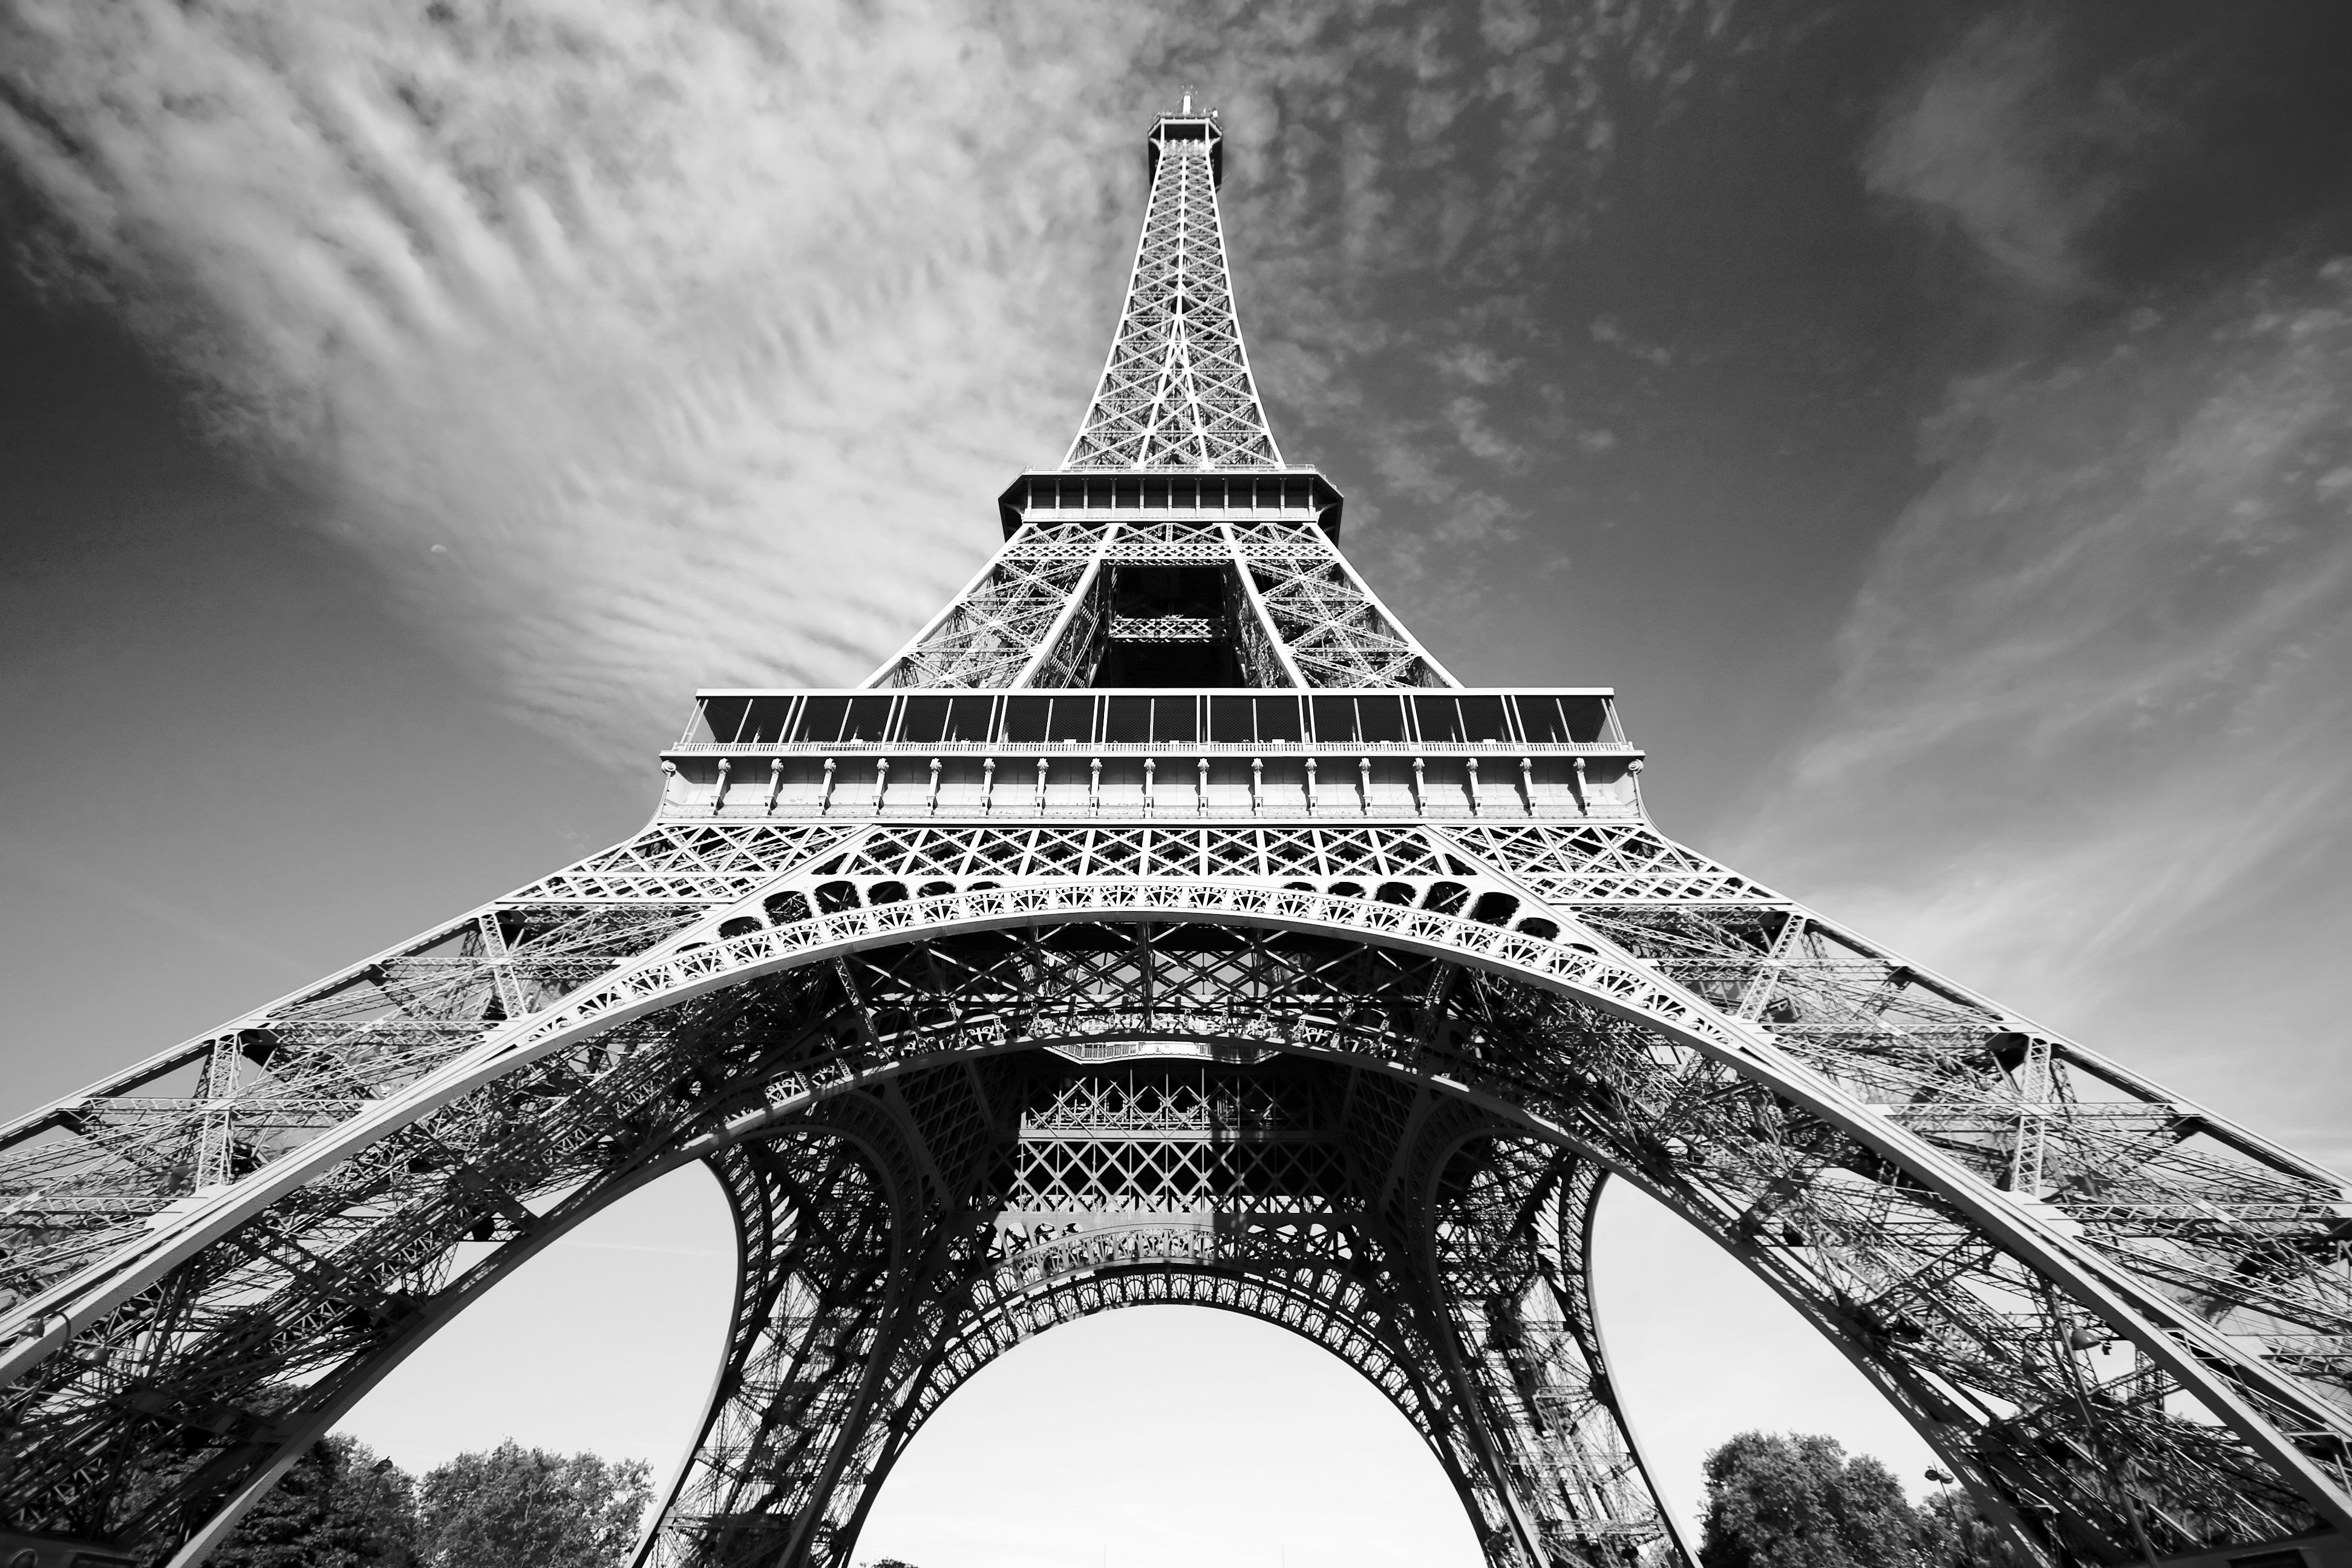
\includegraphics[width=\linewidth]{./img/out.jpg}
    \caption{Histogram equalized}
  \end{subfigure}
\end{figure}

\end{document}
